\chapter{Geladenes Teilchen im elektrischen Feld\label{chapter:efeld}}
\lhead{Teilchen im elektrischen Feld}
\begin{refsection}
\chapterauthor{Michael Cerny und Stefan Schindler}


In diesem Kapitel erweitern wir das Beispiel des Potentialkastens 
(Kapitel \ref{subsection:potentialkasten}, Seite \pageref{subsection:potentialkasten})
um eine St\"orung.

\section{ St"orungstheorie }
Grundsätzlich k"onnen wir mit der St\"orungstheorie ein einfaches Modell mit einer St\"orung erg"anzen, anstatt von Anfang an mit einem komplexen Modell zu rechnen.
Allgemein gilt
\[
f(x, \varepsilon) = f_0(x) + \varepsilon*f_1(x) + \varepsilon^2*f_2(x) + ...
\]
Dabei ist $f_0(x)$ die original Funktion und $f_n(x)$ die n-te  N"aherung der Störung.
Mit $\varepsilon$ wird die Störung gesteuert. Dabei sollte $\varepsilon = 0$ nicht zu gross gew"ahlt werden, weil sonst die N"aherung ungenau wird. $\varepsilon = 0$ bedeutet keine Störung.

In der Quantenmechanik k"onnen wir die St"orungstheorie anwenden indem wir den Hamilton-Operator erg"anzen:
\[
H = \varepsilon^0*H_0 + \varepsilon^1*H_1 + \varepsilon^2*H_2 + ...
\]
Daraus kann die N"aherung der St"orung berechnet werden.



\subsubsection{ Modell der St\"orung }
% TODO

In diesem Modell wollen wir den Grundzustand mit einem elektrischen Feld st\"oren.

Diese St\"orung heisst in der 1. N\"aherung $\hat H_1$

Die gesamte St\"orung wird \"uber den Parameter $\varepsilon$ gesteuert.

$V_1$ wird als lineares Feld definiert:
\[
  V_1 = a*x + b
\]

Der Parameter $a$ steht f\"ur die Feldst\"arke. Da diese jedoch bereits durch 
$\varepsilon$ beschrieben wird, k\"onnen wir die Formel f\"ur $V_1$ mit $a = 1$ vereinfachen:
\[
  \hat{H} = \varepsilon^0 ( \frac{\hbar^2}{2m} \frac{\partial^2}{\partial x^2} + V_0(x) )
            + \varepsilon^1 ( \frac{\hbar^2}{2m} \frac{\partial^2}{\partial x^2} + x )
\]


\begin{figure}
 \centering
 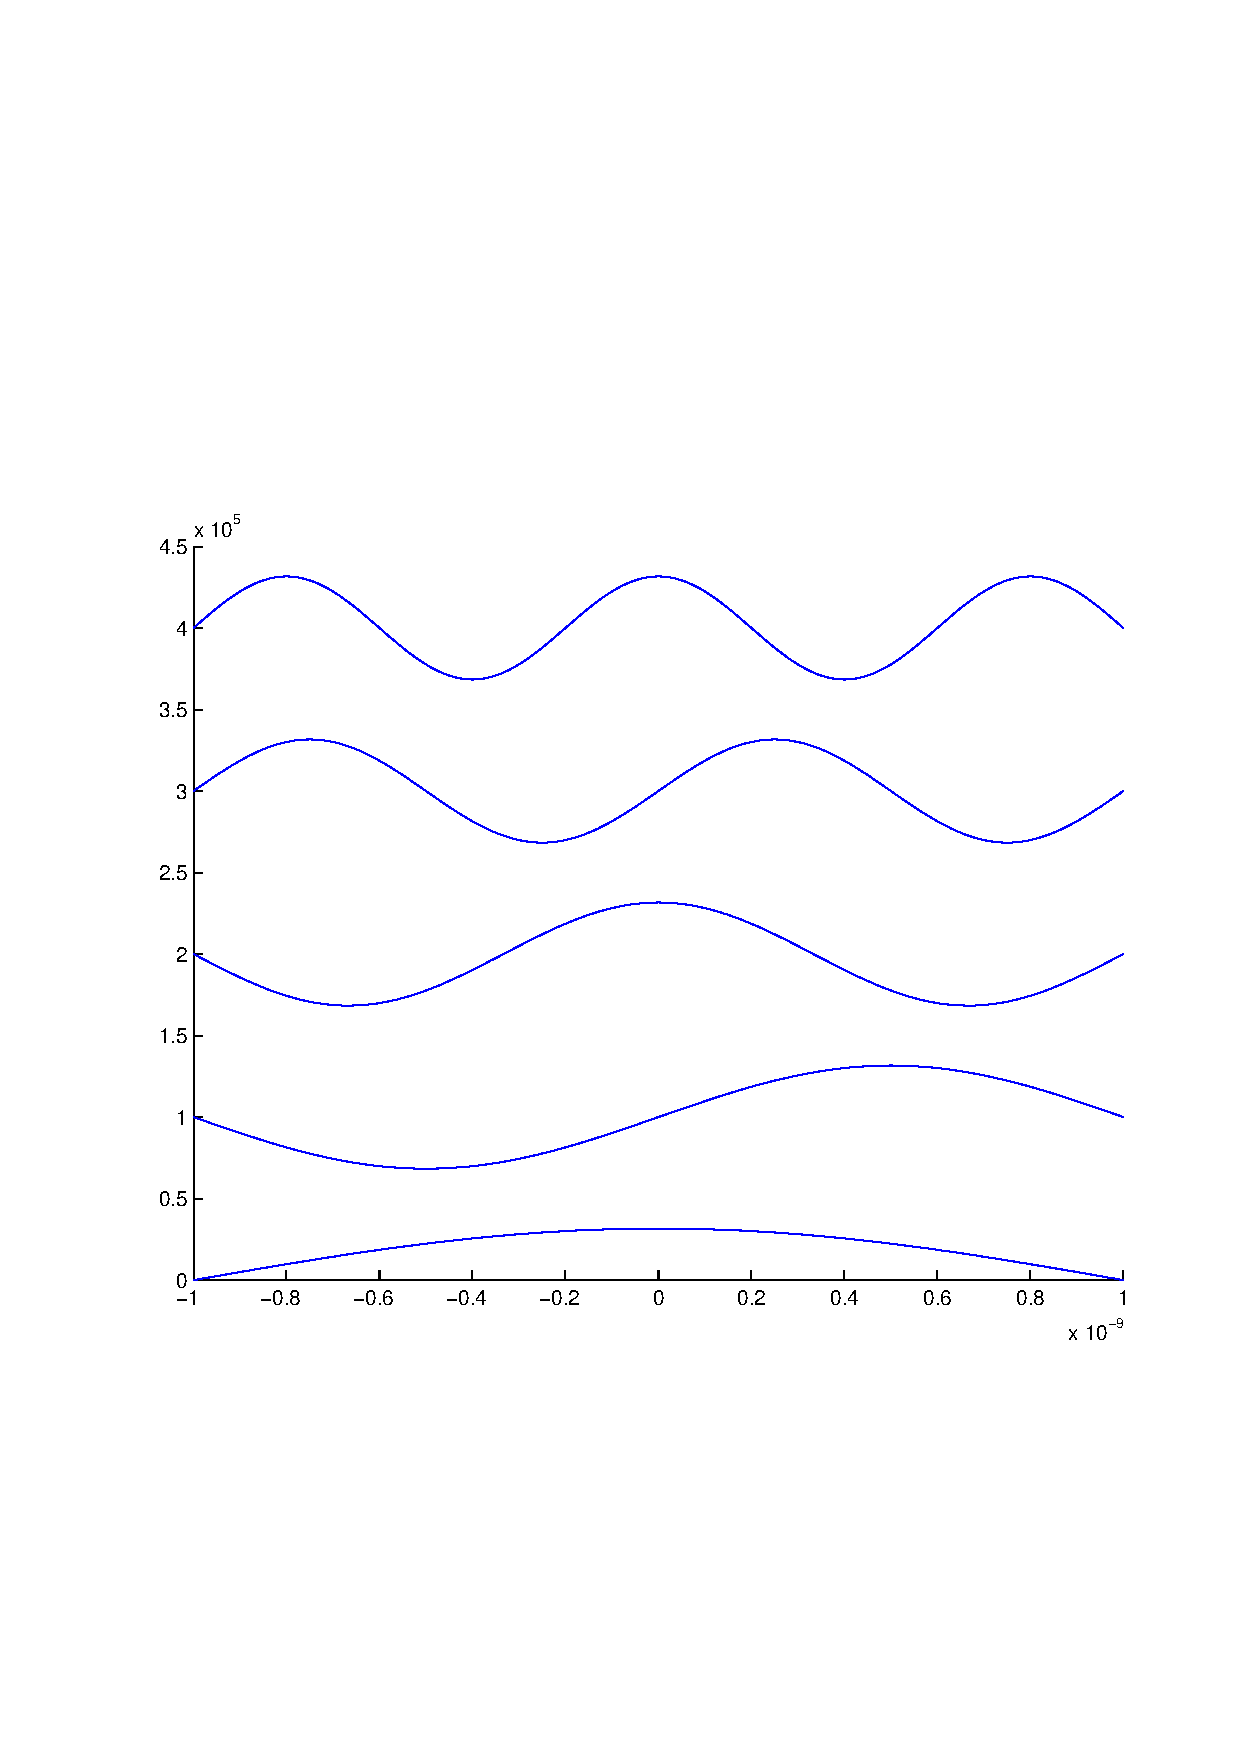
\includegraphics[width=12cm,clip=true,trim=2cm 7cm 1cm 8cm]{efeld/Psi_ungestoert.pdf}
 \caption{$\psi$ ungest\"ort}
 \label{abb:efeld_psi_ungestoert}
\end{figure}




\section{ Beispiele }

\subsection{ Potentialkasten mit eFeld }

Wir berechnen in diesem Beispie die erste N"aherung von einem Potentialskasten mit elektrischem Feld.
Dazu erweitern wir das einfache System  $\hat H_0$
(Siehe Abbildung \ref{skript:potentialkasten})
um $\hat H_1$, welcher die Störung darstellt.
\[
  \hat{H} = \hat H_0 + \varepsilon \hat H_1
\]
F"ur $\hat H_0$ nehmen wir die Funktion aus dem Skript
\[
  \hat H_0 = \frac{\hbar^2}{2m} \frac{\partial^2}{\partial x^2} + V_0(x)
\]
wobei f\"ur das Potential $V_0(x)$ gilt
\[
  V_0(x)=\begin{cases}
    0       & \qquad |x|<l\\
    \infty  & \qquad\text{sonst.}
  \end{cases}
\]

$\hat H_1$ gibt unser elektrisches Feld an
\[
  \hat H_1 = a*x + b
\]
wir k"onnen $b = 0$ setzen da die Potenzials-Barriere unendlich gross ist und $a = 1$ weil wir die St"orung mit $\varepsilon$ steuern.
Die Ausgangsgleichung f\"ur $\hat{H}$ lautet somit
\[
  \hat{H} = \varepsilon^0 ( \frac{\hbar^2}{2m} \frac{\partial^2}{\partial x^2} + V_0(x) )
            + \varepsilon^1*x
\]


\subsection{ 1. N"aherung }

Wie kamen wir darauf?

\begin{enumerate}
\item Gegeben ist eine Gleichung $F_\varepsilon(x)=0$, gesucht
sind die L"osungen $x_\varepsilon$ der Gleichung in Abh"angigkeit von
$\varepsilon$.
\item Die L"osung $x_0$ der Gleichung f"ur den Parameterwert $\varepsilon=0$
ist bekannt.
\item Setze die L"osung in Form einer Potenzreihe an:
$x_\varepsilon = x_0+x_1\varepsilon+x_2\varepsilon^2+\dots$
\item Setze den L"osungsansatz in die Gleichung $F_\varepsilon(x)=0$ ein
und ermittle die Koeffizienten $x_1,x_2,\dots$ durch Koeffizientenvergleich.
\end{enumerate}

In der Grafik \ref{abb:efeld_psi_gestoert} sehen wir die Unterschide zwischen dem normalen $\psi$ (schwarz) \& der ersten N"aherung (rot).

In diesem Beispiel haben wir die Unterschiede mit sehr starken Parmetern gewählt.

Die einzelnen Werte in y-Richtung sind die jeweiligen N"aherungen. Alle Kurven pendeln um die 0-Achse.

\begin{figure}
 \centering
 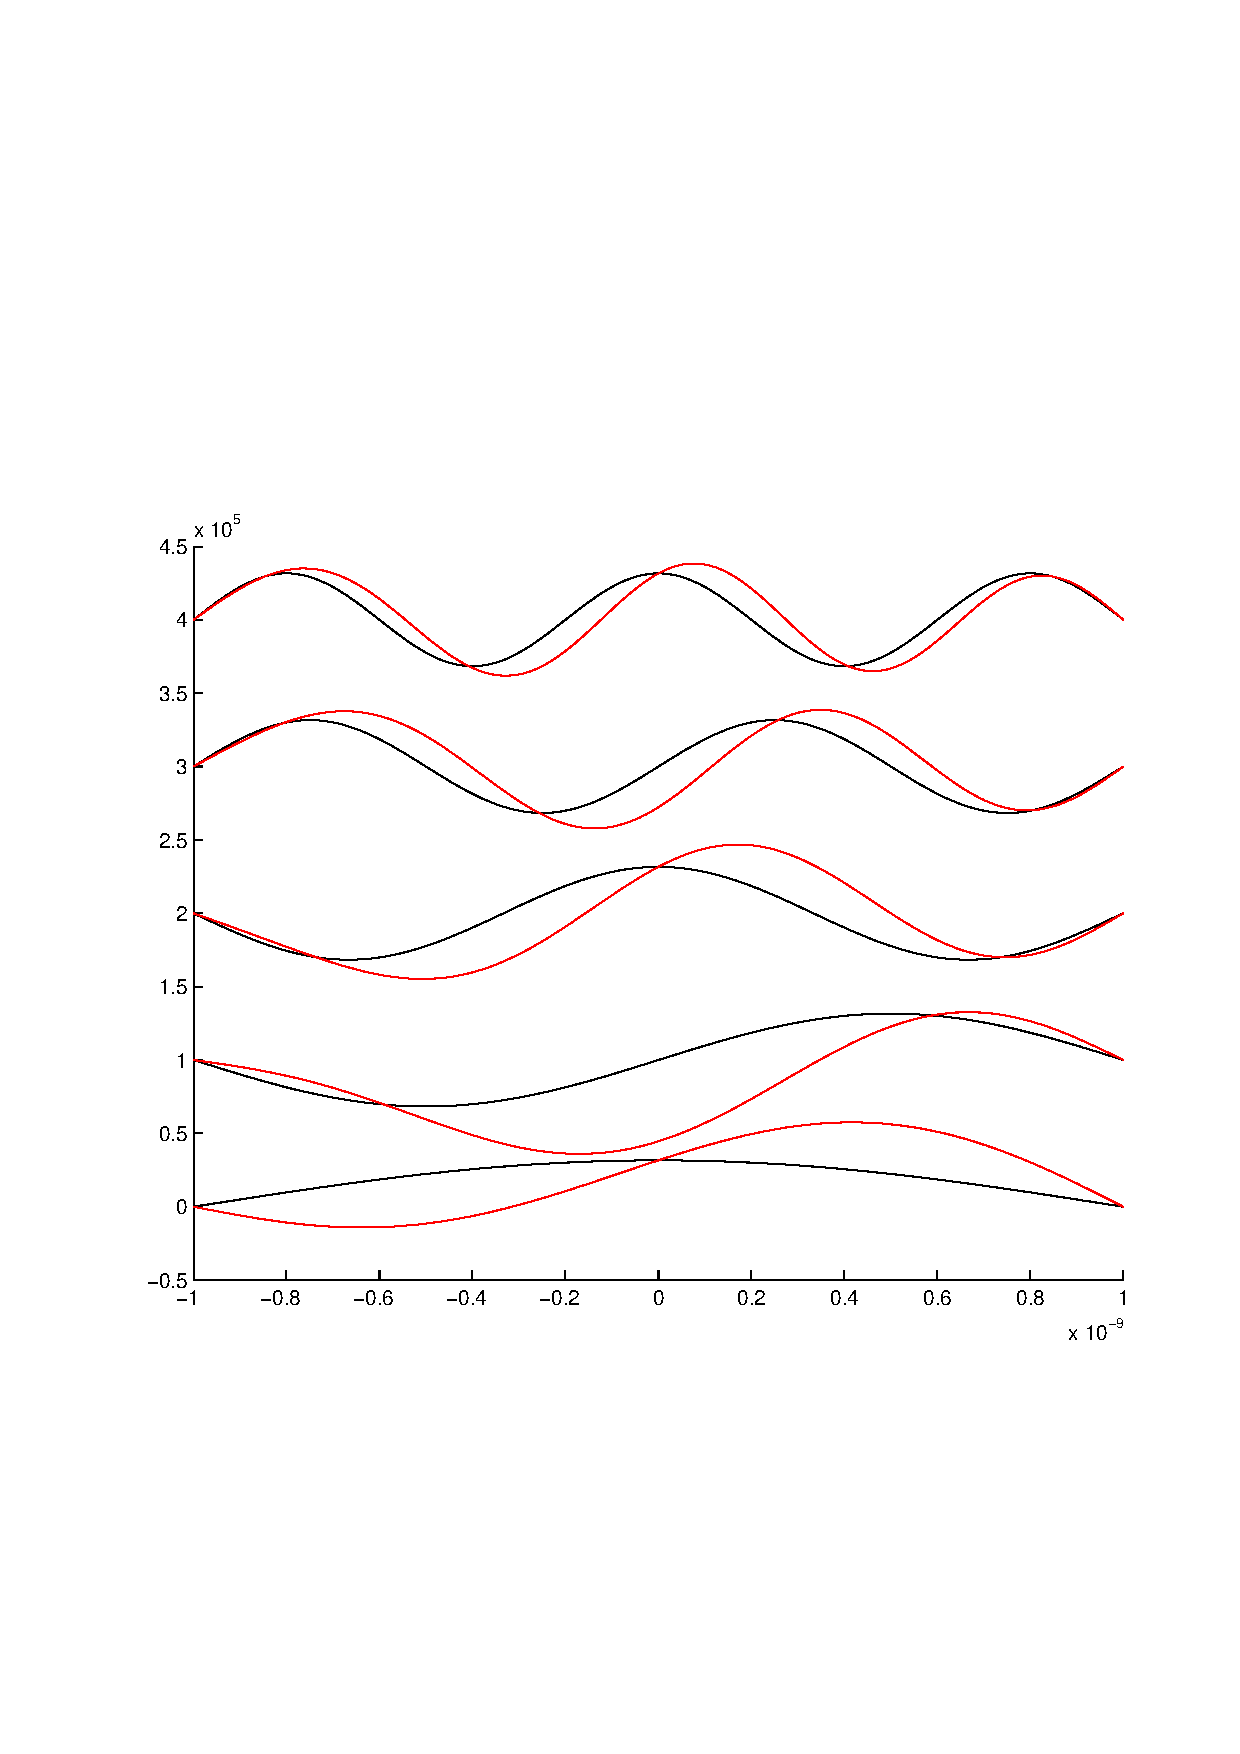
\includegraphics[width=12cm,clip=true,trim=2cm 7cm 1cm 8cm]{efeld/Psi_gestoert.pdf}
 \caption{$\psi$ gest\"ort}
 \label{abb:efeld_psi_gestoert}
\end{figure}


\begin{figure}
 \centering
 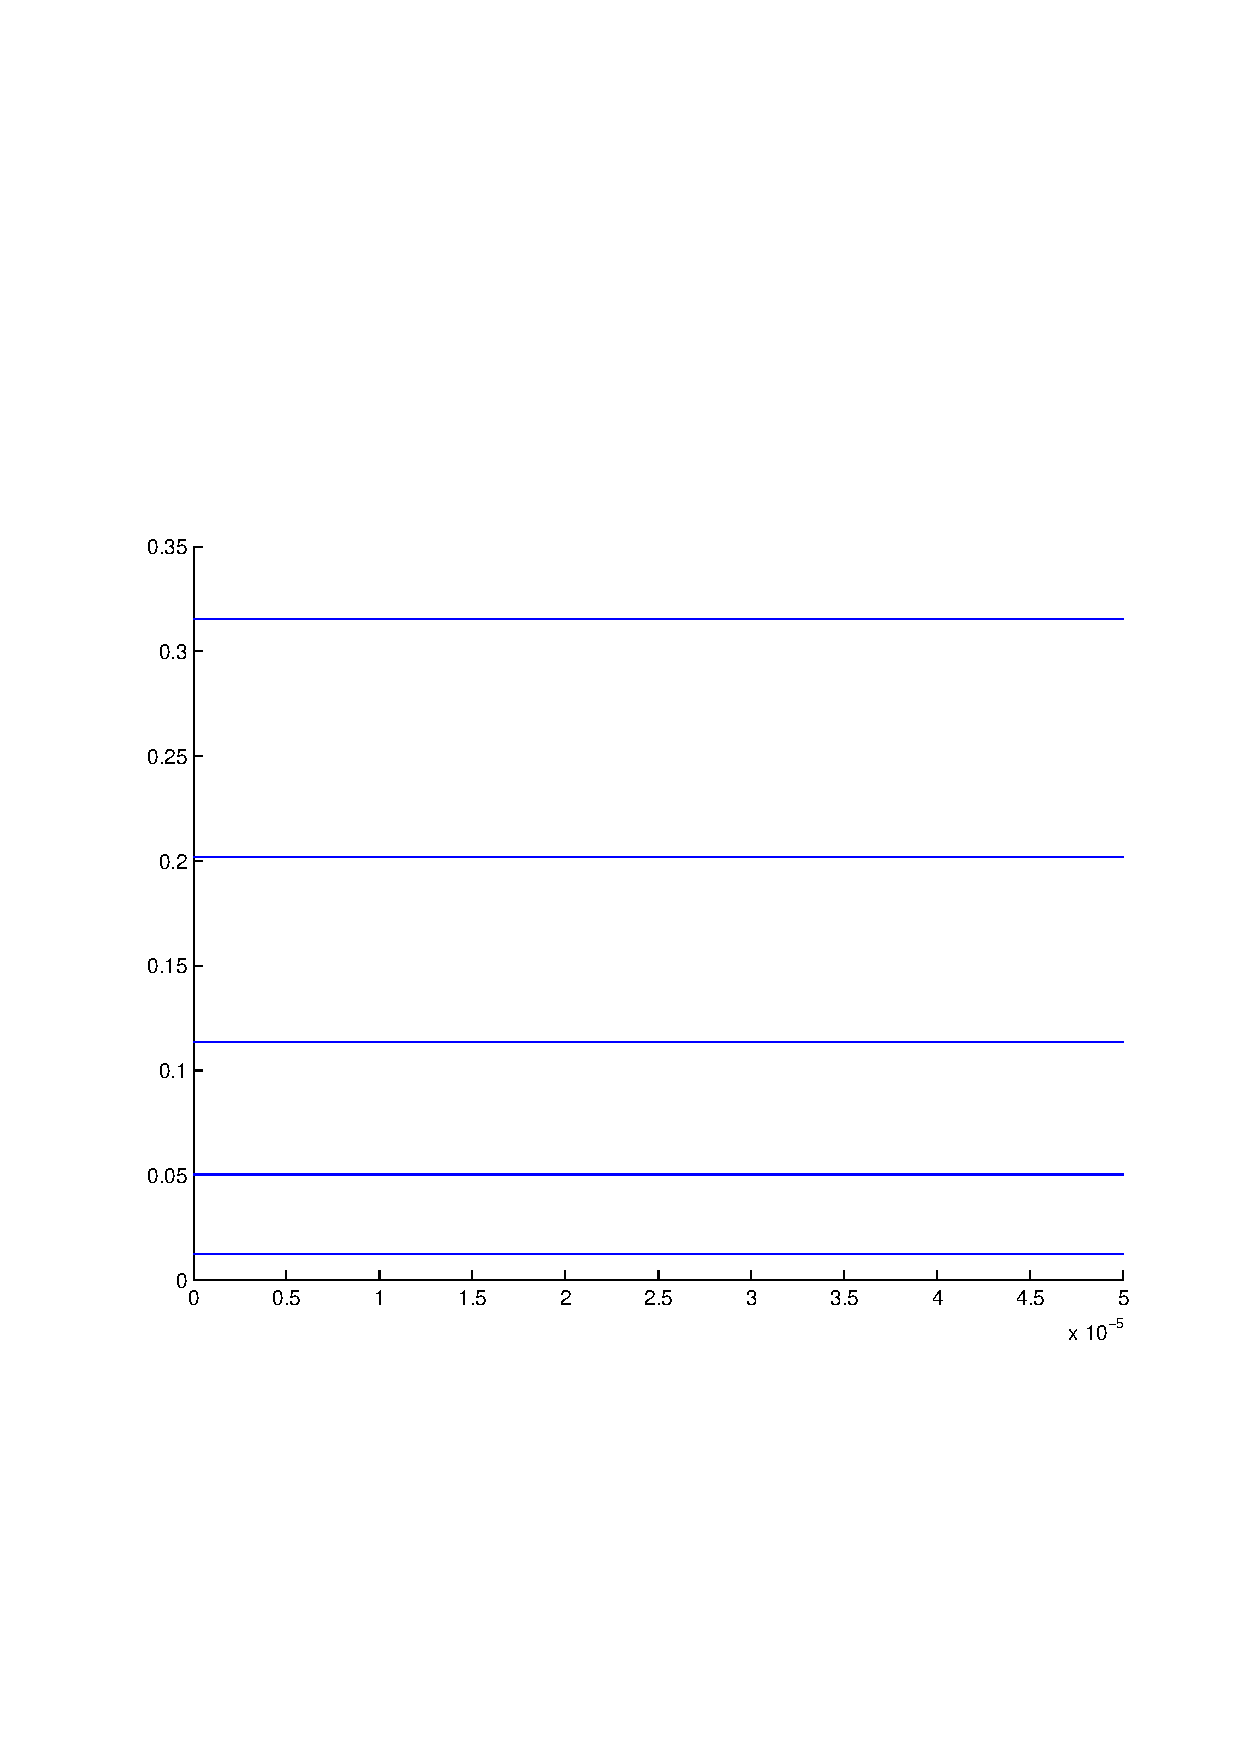
\includegraphics[width=12cm,clip=true,trim=2cm 7cm 1cm 8cm]{efeld/Energie_gestoert.pdf}
 \caption{$E$ gest\"ort}
 \label{abb:efeld_E_gestoert}
\end{figure}



\subsection{ Energie "Anderung }

Was passiert?

\section{ 3. Anwendung Potentialtopf }

\[
  V_1 = \text{ innen \& aussen am Topf ... }
\]
]


\printbibliography[heading=subbibliography]
\end{refsection}
